\documentclass{article}

\usepackage[utf8]{inputenc}
\usepackage{setspace}
\usepackage{geometry}
\usepackage{amsfonts}
\usepackage{booktabs}
\usepackage{tabularx}
\usepackage{caption} 
\usepackage{graphicx}
\usepackage{xcolor}
\usepackage{subcaption}
\usepackage{hyperref}
\usepackage{enumitem}

\usepackage[
    backend=biber,
    style=bwl-FU,
    url=false,
    doi=false,
    eprint=false
]{biblatex}
\addbibresource{article.bib}

\geometry{a4paper,left=1.2in,right=1.2in,top=1in,bottom=1in}

\renewcommand{\baselinestretch}{1.5}
\setlength{\parindent}{0pt}

\title{Final Assignment}
\author{\textup{Shujun Wang\\
                Wenying Huang\\
                Simon Willimann}}

\begin{document}


\begin{titlepage}
	\newcommand{\HRule}{\rule{\linewidth}{0.5mm}}
	
\includegraphics[width=5cm]{uzh_logo.png}\\[1cm] 
	\center 
	\quad\\[1.5cm]
	\textsl{\Large University of Zurich }\\[0.5cm] 
	\textsl{\large Department of Banking and Finance}\\[0.5cm] 
	\makeatletter
	\HRule \\[0.4cm]
	{ \huge \bfseries \@title}\\[0.4cm] 
	\HRule \\[1.5cm]
	\begin{minipage}{0.4\textwidth}
		\begin{flushleft} \large
			\emph{Author:}\\
			\@author 
		\end{flushleft}
	\end{minipage}
	~
	\begin{minipage}{0.4\textwidth}
		\begin{flushright} \large
			\emph{Lecturer:} \\
			\textup{Dr. Igor Pozdeev}
		\end{flushright}
	\end{minipage}\\[3cm]
	\makeatother
	{\large }\\[1cm]
	{\large \emph{21HS DFOEC008 Digital Tools for Finance (L)}}\\[0.5cm]
	{\large \today}\\[2cm] 
	\vfill 
\end{titlepage}

\tableofcontents

\newpage

\section{Introduction}
Numerous scholars have proposed that total stock market returns are predictable\footnote{This is a footnote.}, which provides scope for investors to engage in market timing. At the same time, factors beyond the aggregate market are sources of risk premiums in the cross-section of assets \cite{fama1993common}, creating the basis for
factor investing. 


\section{Literature Review}
There are various papers aim to tackle the entire cross-section, such as \cite{akbas2015smart}, examine the ability of a single variable to forecast all
anomaly returns and thus their common component. Besides, there is a part of the literature on return forecasting studies from the perspective of unsettled factor structures. Better known examples are \cite{lochstoer2020drives} who use panel VAR methods to forecast firm-level expected returns and then construct portfolios. 

\section{Methodology}

\subsection{A subsection}

\textbf{Lemma 1.} (Conditional factor model) This is an equation:

\begin{equation}
\begin{aligned}
\mathbb{E}_{t}\left[R_{j, t+1}\right]=\beta_{j t}^{\prime} \Sigma_{F, t} \delta_{t}=\beta_{j t}^{\prime} \mathbb{E}_{t}\left[F_{t+1}\right] \label{1}
\end{aligned}
\end{equation}

\subsubsection{A sub-subsection}
We use the valuation ratio as a predictor variable and build a forecasting model to obtain the predicted value of each principal component. The valuation ratio is the most commonly used predictor of market returns and, in fact, its use implies an assumption that valuation ratios are believed to provide information about expected returns.

\begin{figure}[h]
\centering
\centering
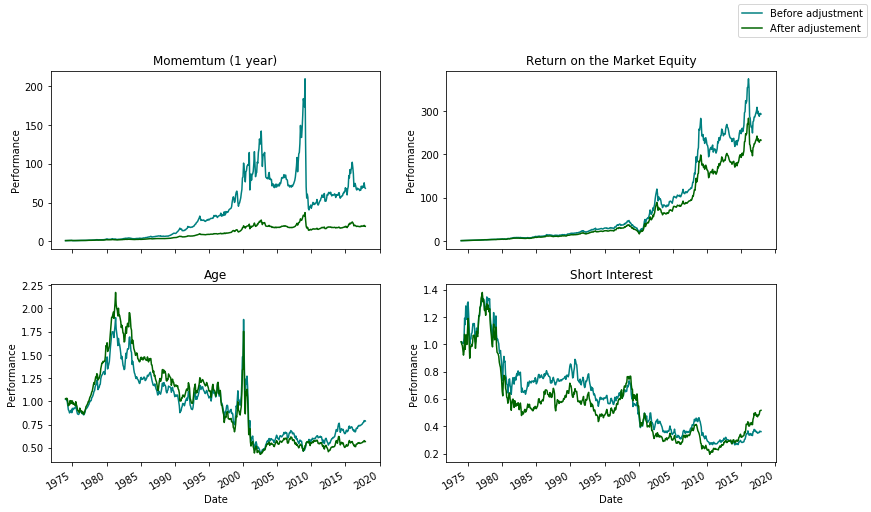
\includegraphics[width=.8\linewidth]{Figure_1.png}
\captionof{figure}{This is a figure. }
\label{Figure 1}
\end{figure}


\begin{table}[h]
\centering
\caption{This is a table. }
\label{Table 1}
\begin{tabular}{lllll}
\toprule
 & Mom12 & rome & age & shortint \\ \hline
 $r$& 10.08 & 13.77 & -0.53 & -2.29 \\
 \sigma& 24.77 & 17.24 & 15.48 & 13.75 \\
 $SR$& 40.68 & 79.91 & -3.48 & -16.66 \\
 $MDD$& -80.70 & -59.96 & -76.39 & -80.64\\
\bottomrule
\end{tabular}
\end{table}


Table \ref{Table 1} shows that the first ten PCs only explain a small portion of the variance compared to \cite{haddad2020factor}, where they demonstrate that nearly the two first PC in other assets classes such as in foreign exchange and Treasury Bond account for nearly 100\% of the variance. 


\section{Conclusion}

In general, factor timing, which combines the concepts of long-short factor investing and market timing, can be extremely beneficial, delivering greater results when compared to market timing and factor investing alone.


\newpage
\printbibliography

\newpage
\section{Appendix}


\begin{figure}[h]
\centering
\begin{minipage}{.5\textwidth}
  \centering
  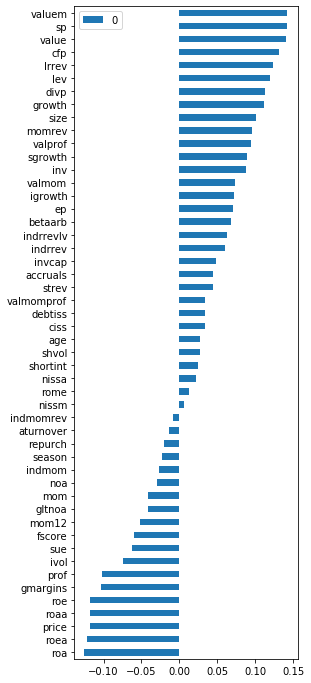
\includegraphics[width=.8\linewidth]{Figure_PC1.png}
  \captionof{figure}{This is a figure}
  \label{eig3}
\end{minipage}%
\begin{minipage}{.5\textwidth}
  \centering
  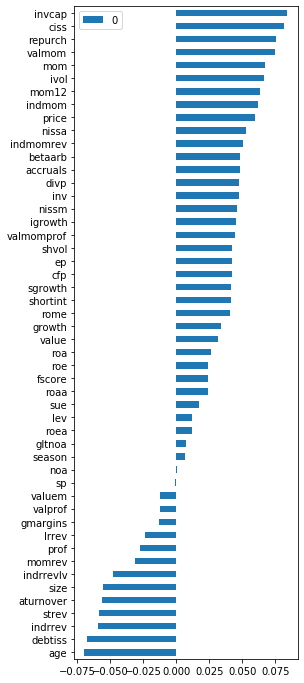
\includegraphics[width=.8\linewidth]{Figure_PC2.png}
  \captionof{figure}{This is another figure}
  \label{eig4}
\end{minipage}
\end{figure}



\end{document}
